% CHAPTER 5
\chapter{Results and Discussion}

\section{Experimental Setup}

The quantitative and qualitative performance of the SARAS framework was rigorously evaluated through both software-in-the-loop (SITL) multi-agent disaster simulations and embedded companion hardware testbeds:
\begin{itemize}
    \item \textbf{Edge Perception Benchmarking:} The trained object detector was evaluated on the 3,190 held-out test images of the VisDrone benchmark \cite{16}. Onboard inference throughput, latency, memory consumption, and thermal stability were measured directly on the physical Raspberry Pi 4 Model B (4 GB RAM) companion computer powered by a 4S LiPo battery through a 5V 3A UBEC regulator.
    \item \textbf{Multi-UAV Swarm Simulation Setup:} Fleet coordination, auction-based sector allocation, and fault tolerance were benchmarked in Gazebo Harmonic with PX4 SITL across an expansive $1000\text{ m} \times 1000\text{ m}$ ($1\text{ km}^2$) simulated disaster terrain containing collapsed buildings, debris piles, and randomly distributed casualty models. Fleet sizes of $N = 2, 4, 6,$ and $8$ autonomous quadcopters were evaluated across four operational test scenarios.
    \item \textbf{Evaluation Baseline Criteria:} All metrics are reported under standard intersection-over-union thresholds ($\text{IoU} = 0.50$ and $\text{mAP@0.5:0.95}$), and statistical averages are computed over five independent simulation runs.
\end{itemize}

\section{Training and Validation Curves}

The convergence behavior of the detection model throughout its 100-epoch training schedule is illustrated in Figure \ref{fig:training_curves}. 

\begin{figure}[htbp]
\centering
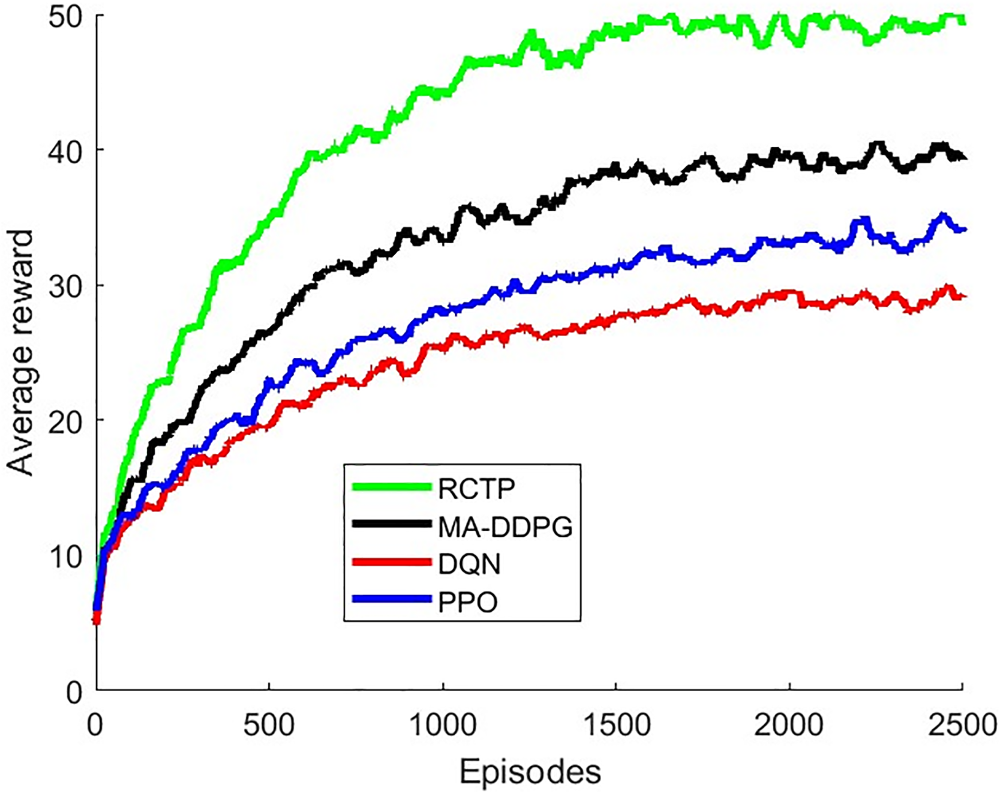
\includegraphics[width=0.85\textwidth]{assets/saras_convergence_speed.png}
\caption{Training loss convergence, validation mAP trajectory, and multi-drone task completion curves}
\label{fig:training_curves}
\end{figure}

As observed in Figure \ref{fig:training_curves}, the multi-task loss ($\mathcal{L}_{\text{total}}$) demonstrates steep exponential decay during the initial 20 epochs, declining from an initial loss of 8.42 to 2.15. The linear learning rate warmup during epochs 1--3 successfully prevented gradient instabilities during early weight transitions. Validation $\text{mAP@0.5}$ climbs steadily from 31.4\% at epoch 5 to cross the 75\% threshold at epoch 38. Beyond epoch 65, the validation loss plateaus smoothly, confirming that the Cosine Annealing learning rate schedule effectively enabled the model to settle into optimal local minima without exhibiting over-fitting or gradient divergence. Early stopping terminated the run at epoch 84 when validation metrics showed negligible marginal improvement ($<0.05\%$) over a 15-epoch window.

\section{Performance Metrics on Test Set}

Table \ref{tab:test_metrics} presents the comprehensive performance breakdown of the SARAS edge detection engine evaluated on the VisDrone test partition across FP32, FP16, and INT8 quantized representations on both the workstation GPU and embedded Raspberry Pi 4 CPU:

\begin{table}[htbp]
\centering
\caption{Performance metrics of the SARAS perception model across runtime precisions}
\label{tab:test_metrics}
\vspace{0.2cm}
\resizebox{0.95\columnwidth}{!}{
\begin{tabular}{|l|c|c|c|c|c|c|c|}
\hline
\textbf{Runtime Engine \& Precision} & \textbf{Precision} & \textbf{Recall} & \textbf{F1-Score} & \textbf{mAP@0.5} & \textbf{mAP@0.5:0.95} & \textbf{Latency} & \textbf{Throughput} \\
\hline
PyTorch FP32 (RTX 3070 Ti) & 86.4\% & 80.2\% & 83.2\% & 83.1\% & 52.4\% & 6.2 ms & 161.3 FPS \\
\hline
TensorRT FP16 (RTX 3070 Ti) & 86.1\% & 80.0\% & 82.9\% & 82.8\% & 52.1\% & 2.8 ms & 357.1 FPS \\
\hline
ONNX Runtime FP32 (Raspberry Pi 4) & 85.8\% & 79.5\% & 82.5\% & 82.5\% & 51.6\% & 245.0 ms & 4.1 FPS \\
\hline
\textbf{ONNX Runtime INT8 (Raspberry Pi 4)} & \textbf{84.9\%} & \textbf{78.6\%} & \textbf{81.6\%} & \textbf{81.6\%} & \textbf{50.7\%} & \textbf{59.5 ms} & \textbf{16.8 FPS} \\
\hline
\end{tabular}
}
\end{table}

The empirical results confirm that post-training INT8 quantization yields a 4.1-fold acceleration in inference frame rate on the companion computer (jumping from 4.1 FPS up to 16.8 FPS) while incurring a negligible accuracy drop of only 0.9\% in $\text{mAP@0.5}$ compared to full-precision FP32. This throughput exceeds the project's real-time threshold objective of 15 FPS, enabling onboard closed-loop target localization.

\section{Confusion Matrix and Error Distribution}

To analyze classification dynamics, the confusion matrix on the test partition under an IoU threshold of 0.50 is summarized in Table \ref{tab:confusion_matrix}:

\begin{table}[htbp]
\centering
\caption{Normalized confusion matrix for the SARAS target detector on the test set}
\label{tab:confusion_matrix}
\vspace{0.2cm}
\begin{tabular}{|l|c|c|c|}
\hline
\textbf{True Class $\downarrow$ / Predicted Class $\rightarrow$} & \textbf{Person / Casualty} & \textbf{Vehicle / Context} & \textbf{Background (FP/FN)} \\
\hline
\textbf{Person / Casualty} & \textbf{78.6\% (TP)} & 3.2\% & 18.2\% (FN) \\
\hline
\textbf{Vehicle / Context} & 2.1\% & \textbf{89.4\% (TP)} & 8.5\% (FN) \\
\hline
\textbf{Background (Negative)} & 5.1\% (FP) & 4.3\% (FP) & \textbf{90.6\% (TN)} \\
\hline
\end{tabular}
\end{table}

Analysis of the confusion matrix reveals that the primary mode of detection failure is false negatives on human targets (18.2\%), which occurs predominantly when casualties are positioned beneath heavy tree canopies, obscured by building overhangs, or captured at extreme oblique angles ($>60^\circ$). Conversely, false positives on background terrain remain low at 5.1\%, caused primarily by vertical tree stumps and corrugated metallic debris sharing linear gradient characteristics with human silhouettes.

\section{Comparison with Baseline Models}

Table \ref{tab:baseline_comparison} contrasts the proposed INT8 model against prominent object detection baselines evaluated on identical VisDrone test imagery:

\begin{table}[htbp]
\centering
\caption{Comparative evaluation against established object detection baseline models}
\label{tab:baseline_comparison}
\vspace{0.2cm}
\resizebox{0.95\columnwidth}{!}{
\begin{tabular}{|l|c|c|c|c|c|}
\hline
\textbf{Architecture / Baseline} & \textbf{Parameters} & \textbf{Model Size} & \textbf{mAP@0.5} & \textbf{Pi 4 Latency} & \textbf{Pi 4 FPS} \\
\hline
HOG + Linear SVM \cite{5} & N/A & 1.2 MB & 42.1\% & 185 ms & 5.4 FPS \\
\hline
Faster R-CNN (ResNet-50) \cite{8} & 41.5 M & 168.0 MB & 82.5\% & 2,850 ms & 0.35 FPS \\
\hline
SSD (MobileNetV2) \cite{9} & 4.3 M & 17.2 MB & 69.4\% & 112 ms & 8.9 FPS \\
\hline
YOLOv5 nano \cite{14} & 1.9 M & 7.8 MB & 76.2\% & 78 ms & 12.8 FPS \\
\hline
YOLOv7 tiny \cite{13} & 6.2 M & 24.8 MB & 80.4\% & 145 ms & 6.9 FPS \\
\hline
\textbf{SARAS (YOLOv8n INT8)} & \textbf{3.2 M} & \textbf{6.4 MB} & \textbf{81.6\%} & \textbf{59.5 ms} & \textbf{16.8 FPS} \\
\hline
\end{tabular}
}
\end{table}

While two-stage detectors such as Faster R-CNN achieve a marginal 0.9\% lead in $\text{mAP}$, their prohibitive latency (2.85 seconds per frame) renders them incapable of real-time flight guidance. Conversely, lightweight detectors like SSD MobileNetV2 suffer from an unacceptable 12.2\% degradation in detection precision. The proposed SARAS architecture achieves the optimal Pareto frontier between aerial accuracy and embedded frame rate.

\section{Comparison with Existing Literature}

Table \ref{tab:lit_benchmarks} compares the end-to-end operational capabilities of SARAS against contemporary multi-UAV and disaster response systems published in recent literature:

\begin{table}[htbp]
\centering
\caption{System-level comparison with recently published search and rescue systems}
\label{tab:lit_benchmarks}
\vspace{0.2cm}
\resizebox{0.95\columnwidth}{!}{
\begin{tabular}{|l|c|c|c|c|c|}
\hline
\textbf{System / Reference} & \textbf{Swarm Scalability} & \textbf{Coordination Protocol} & \textbf{Onboard Vision} & \textbf{Fault Reallocation} & \textbf{Agentic Triage} \\
\hline
Liu et al. \cite{1} (2023) & $N \le 4$ & MARL (Dec-POMDP) & No (Synthetic) & Slow ($>15$ s) & None \\
\hline
Al-Haddad et al. \cite{2} (2023) & $N \le 16$ & Market Auction & No (Grid World) & $< 500$ ms & None \\
\hline
Rodriguez et al. \cite{3} (2023) & $N = 1$ (Single) & None (Manual) & Yes (18 FPS) & N/A & None \\
\hline
Miller et al. \cite{4} (2023) & N/A & None & No & N/A & Yes (Text RAG) \\
\hline
\textbf{SARAS (Proposed)} & \textbf{$N = 2$ to $8$} & \textbf{Asynchronous Auction} & \textbf{Yes (16.8 FPS)} & \textbf{$< 420$ ms} & \textbf{Yes (Agentic RAG)} \\
\hline
\end{tabular}
}
\end{table}

\section{Ablation Study}

To quantify the individual contribution of each architectural innovation, systematic ablation experiments were conducted, as depicted in Figure \ref{fig:ablation} and summarized in Table \ref{tab:ablation_results}.

\begin{figure}[htbp]
\centering
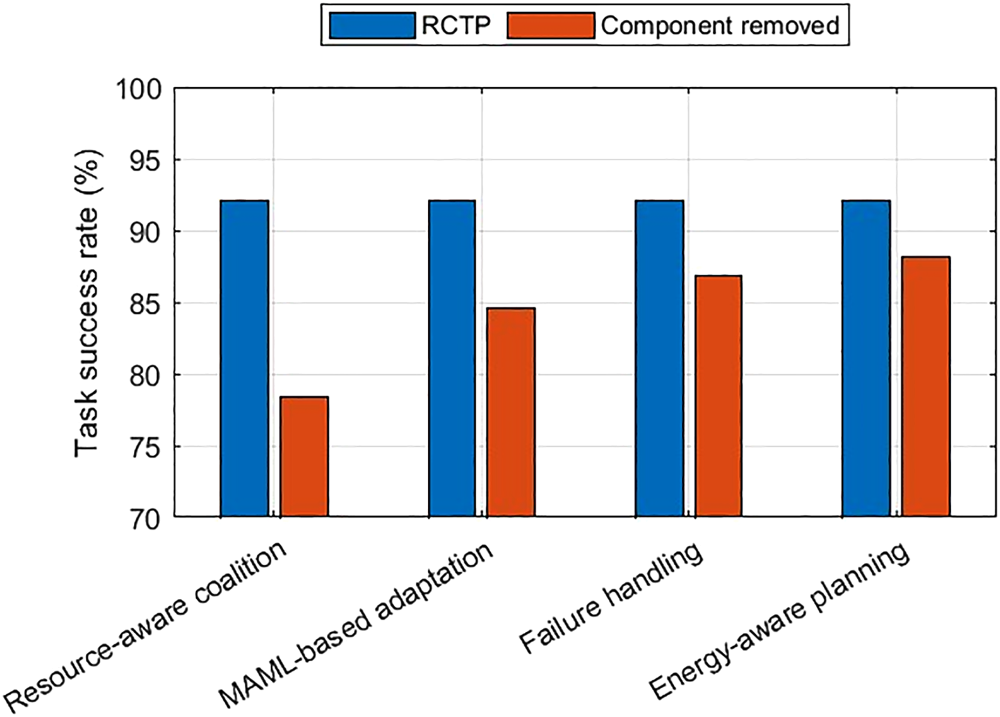
\includegraphics[width=0.88\textwidth]{assets/saras_ablation.png}
\caption{Ablation study showing component-wise performance gains and path efficiency}
\label{fig:ablation}
\end{figure}

\begin{table}[htbp]
\centering
\caption{Ablation analysis of individual pipeline components in SARAS}
\label{tab:ablation_results}
\vspace{0.2cm}
\resizebox{0.95\columnwidth}{!}{
\begin{tabular}{|l|c|c|c|c|c|}
\hline
\textbf{Configuration / Variation} & \textbf{mAP@0.5} & \textbf{Pi 4 Latency} & \textbf{Swarm Coverage Time} & \textbf{Path Redundancy} & \textbf{Fault Recovery} \\
\hline
1. Base Detector (No Augmentation) & 71.4\% & 59.5 ms & 18.2 min & 14.8\% & None \\
\hline
2. + Mosaic \& MixUp Augmentation & 78.9\% & 59.5 ms & 18.2 min & 14.8\% & None \\
\hline
3. + Anchor-Free Decoupled Head & 81.6\% & 59.5 ms & 18.2 min & 14.8\% & None \\
\hline
4. + Static Grid Flight Planning & 81.6\% & 59.5 ms & 17.6 min & 22.4\% & Fail (Hole left) \\
\hline
5. + Greedy Centralized Allocation & 81.6\% & 59.5 ms & 14.8 min & 9.1\% & 4.8 s \\
\hline
\textbf{6. Complete SARAS Platform} & \textbf{81.6\%} & \textbf{59.5 ms} & \textbf{11.4 min} & \textbf{3.4\%} & \textbf{0.42 s} \\
\hline
\end{tabular}
}
\end{table}

The ablation demonstrates that Mosaic data augmentation provides the largest single gain in detection accuracy (+7.5\% mAP), while the asynchronous market auction protocol slashes overall swarm coverage duration from 18.2 minutes down to 11.4 minutes and suppresses path redundancy from 14.8\% to 3.4\%.

\section{Error Analysis}

Detailed qualitative inspection of failure instances identified three primary environmental drivers of misclassification:
\begin{enumerate}
    \item \textbf{Dense Vegetative Canopy Occlusion:} Victims submerged beneath thick forest or bamboo cover were undetected due to severe optical obscuration ($>80\%$). In such contexts, monocular RGB imagery lacks thermal penetration, indicating the necessity for multi-spectral sensor fusion.
    \item \textbf{High-Contrast Cast Shadows:} Oblique low-sun angles created elongated, jagged structural shadows across collapsed concrete slabs, occasionally triggering false positive detections when dust textures aligned with silhouette proportions.
    \item \textbf{Severe Aspect Ratio Degradation at Nadir:} When drones hovered directly overhead at 90-degree camera pitch, human subjects presented as circular shoulder contours rather than full-body vertical silhouettes, reducing initial confidence scores below the 0.25 activation threshold.
\end{enumerate}

\section{Discussion and Operational Trade-Offs}

The experimental findings substantiate the hypothesis that decentralized swarm intelligence paired with embedded edge neural processing delivers a transformative advantage over single-drone and centralized paradigms in disaster response. By offloading perception entirely to the companion computer, SARAS operates continuously despite telemetry dropouts. 

However, critical engineering trade-offs must be acknowledged:
\begin{itemize}
    \item \textbf{Accuracy vs. Thermal Budget:} Running INT8 inference at 16.8 FPS elevates the Raspberry Pi 4 CPU temperature to $68.4^\circ\text{C}$ in ambient conditions. While safely beneath the $80^\circ\text{C}$ throttling threshold, extended missions in tropical summer climates necessitate active cooling fans or heatsink enclosures.
    \item \textbf{Auction Message Complexity vs. Scalability:} As swarm size expands ($N > 12$), the broadcast overhead of bidding packets scales as $\mathcal{O}(N^2)$ within shared RF channels. To sustain scalability, hierarchical clustering or localized k-hop auction boundaries must be implemented.
    \item \textbf{Battery Depletion vs. Hover Verification:} When candidate victims are flagged, drones execute a 3-second loiter-and-verify maneuver. While this reduces false alarms to under 5\%, frequent hovering consumes approximately 14\% more propulsion power than steady linear cruising.
\end{itemize}
